\item \textbf{Investiga qué versión del kernel tienes, añadiendo una captura que la muestre en el reporte}  \vspace{0.3cm}

El Kernel que tengo se puede ver en la captura correspondiente:

\begin{figure}[H]
    \centering
    
\includegraphics[width=\textwidth]{src/Img/1.png}
    \caption{uname del sistema}
    \label{fig:kernel}
\end{figure}

Se hacen algunos pasos adicionales que se ven algo asi:

\begin{figure}[H]
    \centering
    
\includegraphics[width=\textwidth]{src/Img/2.png}
    \caption{pasos extra}
    \label{fig:extra}
\end{figure}

Para cambiar el nombre del nuevo kernel lo hice medio manualmente, use estos comandos y dentro del archivo cambie donde dice el UTS SYSNAME:

\begin{figure}[H]
    \centering
    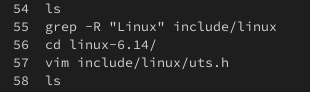
\includegraphics[width=\textwidth]{src/Img/3.png}
    \caption{Cambiandole el nombre al kernel uwu}
    \label{fig:nombre}
\end{figure}

Cabe destacar que cuando estaba haciendo la compilación del kernel usando make se tardo un monton y ademas lo tuve que reiniciar varias veces porque gnome lo detenia por usar demasiados recursos. Ademas le tuve que dar mas cores y mas memoria ram ademas de un HDD mas grande. \vspace{.2cm}

Recomiendo si lo van a hacer usen al menos 30gb de HDD y 4gb de RAM. \vspace{.2cm}

Despues de horas de intentarlo y que regresara errores a la media hora, logre hacer la compilación, aqui una imagen de despues cuando ya complete todos los pasos instalando y otra ya con el nombre cambiando del kernel:

\begin{figure}[H]
    \centering
    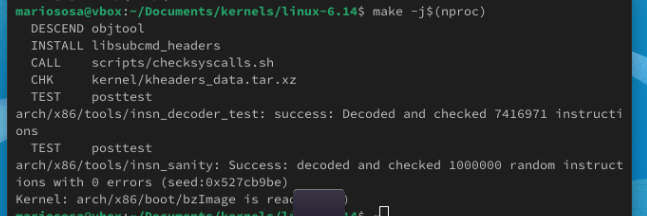
\includegraphics[width=\textwidth]{src/Img/4.png}
    \caption{Compilado}
    \label{fig:compilado}
\end{figure}

\begin{figure}[H]
    \centering
    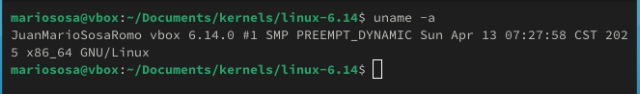
\includegraphics[width=\textwidth]{src/Img/5.png}
    \caption{Final}
    \label{fig:final}
\end{figure}


\section*{Preguntas}
\textbf{¿Qué es el bootloader?}\vspace{.2cm}

El \textit{bootloader} es un programa que se ejecuta justo despues del UEFI o BIOS, se busca en su lugar pre definido en memoria y cabe destacar es un lugar bastante pequeño comparado al kernel desde donde se dedicara a hacer principalmente configuraciones e inicializar el Kernel y el SO, de manera resumida, ajusta el estado del HW para que sea compatible con el Kernel y todo funcione bien, despues de esto el Kenel es quien toma el control. \vspace{.3cm}

\textbf{¿Qué son los kernel modules?}\vspace{.2cm}

Los \textit{kernel modules} son pedazos de codigo que pueden ser cargados y descargados del nucleo sin necesidad de reiniciar el sistema, con ellos podemos personalizar y ampliar las capacidades del kernel de manera dinamica haciendo nuestro sistema flexible y adaptable. \vspace{.2cm}

Los mas comunes de estos son los \textit{drivers} que nos ayudan a gestionar y comunicarnos con el hardware, aunque tambien existen por ejemplo para almacenamiento externo como usbs o red.    